\section{Variante de l'heuristique dans le cas 3x3}\label{appendice:calcul-theorique}

Le contributeur effectue une nouvelle comparaison entre $E_{1}$ et $E_{3}$ avec une notation $n_{1-3} \in [\![-10;10]\!]$. Les scores sont cette fois-ci calculés par l'heuristique.

\begin{align*}
r_{t+1}= \begin{pmatrix}
0 & n_{1-2} &  n_{1-3} \\
-n_{1-2} & 0 & 0\\
 -n_{1-3}  & 0 & 0
\end{pmatrix}
~~~~~~
l_{t+1}= \begin{pmatrix}
0 & l_1 & l_2\\
-l_1 & 0 & 0\\
-l_2 & 0 & 0
\end{pmatrix}
~~~~~~
k_{t+1}= \begin{pmatrix}
0 & k_1 &  k_2 \\
k_1 & 0 & 0 \\
 k_2 & 0 & 0
\end{pmatrix}
\end{align*}

\begin{align*}
l_{t+1} \cdot k_{t+1}= \begin{pmatrix}
0 & l_1 k_1 & l_2 k_2\\
-l_1 k_1 & 0 & 0\\
-l_2 k_2 & 0 & 0
\end{pmatrix}
\end{align*}

\begin{align*}
L_{t+1}= \begin{pmatrix}
l_1 k_1 +l_2 k_2 \\
-l_1 k_1\\
-l_2 k_2
\end{pmatrix} \triangleq
\begin{pmatrix}
L1\\
L2\\
L3
\end{pmatrix} 
~~~~~~
K_{aa,t+1}= \begin{pmatrix}
\alpha + k_1 + k_2\\
\alpha +  k_1 \\
\alpha + k_2
\end{pmatrix} \triangleq
\begin{pmatrix}
K1\\
K2\\
K3
\end{pmatrix} 
\end{align*}




Pour $\tau=0, A^{t+1,0}=\set{E_1,E_3}$

\begin{align*}
  \scoreh_{t+1,0}= \begin{pmatrix}
(L_1+\score_{2} k_1) / K_1 \\
(L_3+\score_{1} k_2) / K_3
\end{pmatrix}  
\end{align*}

avec $\score_{1} = - \score_{2} = l_1 k_1/(\alpha + 2 k_1)$

Pour $\tau=1, A^{t+1,1}=\set{E_1,E_2,E_3}$

\begin{align*}
\scoreh_{t+1,1}= \begin{pmatrix}
(L_1+\score_{2} k_1 + \scoreh_{t+1,0,3} k_2) / K_1 \\
(L_2+\scoreh_{t+1,0,1} k_1) / K_2 \\
(L_3+\scoreh_{t+1,0,1} k_2) / K_3 
\end{pmatrix}    
\end{align*} 


\begin{align*}
 BSN =
(L_1+\score_{2} k_1 + \scoreh_{t+1,0,3} k_2) / K_1 +
(L_2+\scoreh_{t+1,0,1} k_1) / K_2 +
(L_3+\scoreh_{t+1,0,1} k_2) / K_3 
\end{align*}

\begin{equation*}
    \forall{n_{1-2},n_{1-3}}\in [\![-10;10]\!]² , BSN \in [-1.10,1.10]
\end{equation*}

\begin{figure}[ht]
  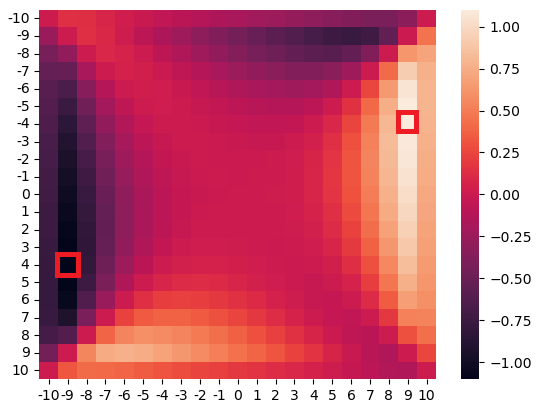
\includegraphics[width=\linewidth]{heatmap2.png}
  \caption{Distribution des résultats de l'indicateur BSN (ordonnée,abscisse)}
  % \vspace{-15pt}
\end{figure}

Le minimum et le maximum sont atteints respectivement en $(n_{1-2},n_{1-3})=(4, -9)$ et en (-4, 9).


Les scores de l'algorithme Mehestan sont données par les formules suivantes :

$K_{t+1} \score_{t+1}= L_{t+1}$

$\score_{t+1}=K^{-1}_{t+1} L$

avec 
$ K_{t+1}= \begin{pmatrix}
K_1&-k_{12}&-k_{13}\\
-k_{12}&K_2&-k_{23}\\
-k_{13}&-k_{23}&K_3
\end{pmatrix}$

ici, $k_{12}=k_1, k_{13}=k_2, k_{23}=0$
alors, 

$ K_{t+1}= \begin{pmatrix}
K_1&-k_1&-k_2\\
-k_1&K_2&0\\
-k_2&0&K_3
\end{pmatrix}$

$ K^{-1}_{t+1}= \left( \begin{array}{ccc} K_1 K_2 & k_1 K_2 & k_2 K_1 \\ k_1 K_2 & K_2 K_3-k_2^2 & k_1 k_2 \\ k_2 K_1 & k_1 k_2 & K_1 K_3-k_1^2 \end{array} \right)/(-K_2 k_1^2-k_2^2 K_1+K_1 K_2 K_3)$

EAM=  $|\score_{t+1,1} - \scoreh_{t+1,1,1}|   +  |\score_{t+1,2} - \scoreh_{t+1,1,2}|  +  |\score_{t+1,3} - \scoreh_{t+1,1,3}|  $



\begin{equation*}
\forall{n_{1-2},n_{2-3}}\in [\![-10;10]\!]²,  EAM \in [0.000,1.640 ]
\end{equation*}


Le minimum et le maximum sont atteints respectivement en $(n_{1-2},n_{1-3})=(0, 0)$ et en (-9, 7).
